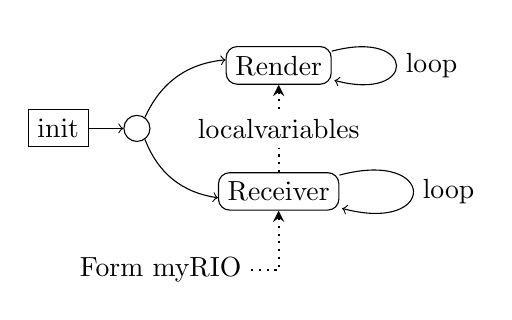
\begin{tikzpicture}
\tikzstyle{rounded} = [rectangle, rounded corners , minimum width=3mm, minimum height=1mm,text centered, draw=black]
\tikzstyle{round}=[circle, minimum width=0mm,draw=black]
\tikzstyle{square} = [rectangle, minimum width=1mm, draw=black]
\tikzstyle{empty}=[]

\usetikzlibrary{shapes.geometric, arrows}
\tikzstyle{arrow} = [thick,->,>=stealth]
\tikzstyle{dottarrow} = [thick, dotted,->,>=stealth]
\tikzstyle{dottline} = [thick, dotted,-,>=stealth]
\tikzstyle{noarrow}=[thick,-=,=stealth]

%nodes
\node (init) [square] {init};
\node (loop) [round, right of=init]{};
\node (render)[rounded, right of=loop, xshift=8mm, yshift=8mm ] {Render};
\node (rezive) [rounded, right of=loop, xshift=8mm, yshift=-8mm] {Receiver};
\node (datain) [empty, below of=rezive, xshift=-15mm]{Form myRIO};
\node (shared) [empty, below of=render, yshift=2mm]{localvariables};


%lines
%(Startnode)  edge [bend arrow]       node[text pos]  {text}          (target);
\path[->] 
(init) 		edge 								node[left]		{}			(loop)
(loop)		edge[bend left] 					node[left]		{}			(render)
(loop)		edge[bend right]					node[left]		{}			(rezive)
(render) 	edge[loop right]					node[right]		{loop}			(render)
(rezive) 	edge[loop right]					node[right]		{loop}			(rezive)
;
\draw [dottarrow] (datain) -| (rezive);
%\draw [dottarrow] (rezive) -- (render);
\draw [dottline] (rezive) -- (shared);
\draw [dottarrow] (shared) -- (render);

\end{tikzpicture}